\documentclass[12pt,a4paper]{article}
\usepackage[margin=1in]{geometry}
\usepackage{graphicx}
\usepackage{float}
\usepackage{caption}
\usepackage{setspace}
\usepackage{booktabs}
\usepackage{hyperref}
\usepackage{enumitem}
\usepackage{xcolor}
\usepackage{listings}
\usepackage{microtype}
\hypersetup{colorlinks=true, linkcolor=black, urlcolor=blue}
\onehalfspacing
\setlength{\parindent}{0pt}
\setlength{\parskip}{0.7em}

\lstdefinestyle{pythonstyle}{
  language=Python,
  basicstyle=\ttfamily\small,
  breaklines=true,
  frame=single,
  columns=fullflexible,
  showstringspaces=false,
  commentstyle=\color{gray},
  keywordstyle=\color{blue!70!black},
  stringstyle=\color{green!40!black}
}

\begin{document}

\begin{titlepage}
\centering
\vspace*{1.4cm}
{\large In the Name of God\\[1.0cm]}
{\large School of Management and Economics\\[0.4cm]}
{\large Financial Economics I\\[1.4cm]}
{\LARGE\bfseries Python Coding Project Report\\[1.3cm]}
{\large Course Instructor:\\[0.2cm] Dr. Mostafa Seraj\\[1.0cm]}
{\large Prepared by:\\[0.2cm] Omid Karami, 400203402\\[2.0cm]}
{\large August 2023}
\vfill
\end{titlepage}

\section*{Question 1}

\subsection*{Part (a)}
First, the required modules for this question and the following questions were imported. Then, the price data for five cryptocurrencies - Bitcoin, Ethereum, Binance Coin, Ripple, and Cardano - during 2022 were downloaded using Yahoo Finance. After that, the price data were normalized by subtracting the mean price of each cryptocurrency over the year and dividing the result by the standard deviation of that cryptocurrency's price.

To make the comparison easier, the price of each cryptocurrency on all days was divided by its price on the first day of 2022. The price trends over time were then plotted for all five cryptocurrencies.

\begin{figure}[H]
\centering
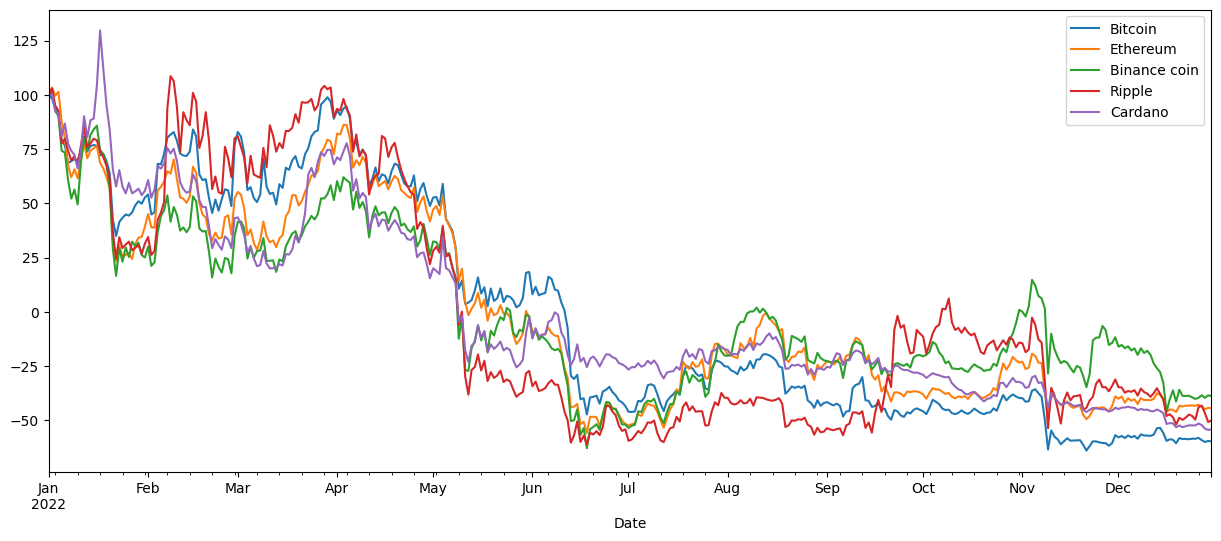
\includegraphics[width=0.98\textwidth]{../figures/notebook_cell5_output0.png}
\caption{Price changes of five cryptocurrencies in 2022}
\end{figure}

As shown in Figure 1, all five cryptocurrencies had negative returns in 2022, and their prices declined relative to the beginning of the year. In absolute terms, Binance Coin had the smallest negative return, while Bitcoin had the largest negative return. According to the question, profitability should also be evaluated using the cumulative return of each cryptocurrency. Using the formula given in the question, the cumulative return of each asset was calculated, and the comparison leads to the same conclusion that is visible in the figure.

\subsection*{Part (b)}
The price data for the selected ten cryptocurrencies over the previous six months were downloaded. Then, the daily return of each cryptocurrency was calculated. Next, by identifying the days on which Bitcoin had a positive daily return and the days on which it had a negative daily return, we observed that the cumulative return of the other cryptocurrencies was positive when Bitcoin's daily return was positive. The same logic applies when Bitcoin's daily return was negative.

The highest positive cumulative return belonged to Solana, and the lowest belonged to Binance Coin. For the negative-return case, if we look at the absolute values, the largest negative return belonged to Solana, while the smallest belonged to Tronix. In this part, the number of days with positive and negative returns was also calculated for each cryptocurrency, including Bitcoin and the altcoins. These results are provided in the code.

\section*{Question 2}

\subsection*{Part (a)}
The price data for Bitcoin, Ethereum, and Ripple in 2022 were downloaded. Then, the daily logarithmic return of each asset was calculated. By averaging across 363 days, the annual return of each cryptocurrency was obtained.

Next, it was assumed that a portfolio could be formed using these three cryptocurrencies, with the condition that the percentage weight of each asset in the portfolio must be a multiple of 5 percent. After calculating the possible weights, the return and volatility of the different portfolio combinations were computed.

\subsection*{Part (b)}
In this part, the return-versus-risk graph was plotted for all possible portfolio weight combinations. These portfolios have different Sharpe ratios\footnote{Sharpe ratio.}, and the graph helps us observe the efficient frontier\footnote{Efficient frontier.} visually.

\begin{figure}[H]
\centering
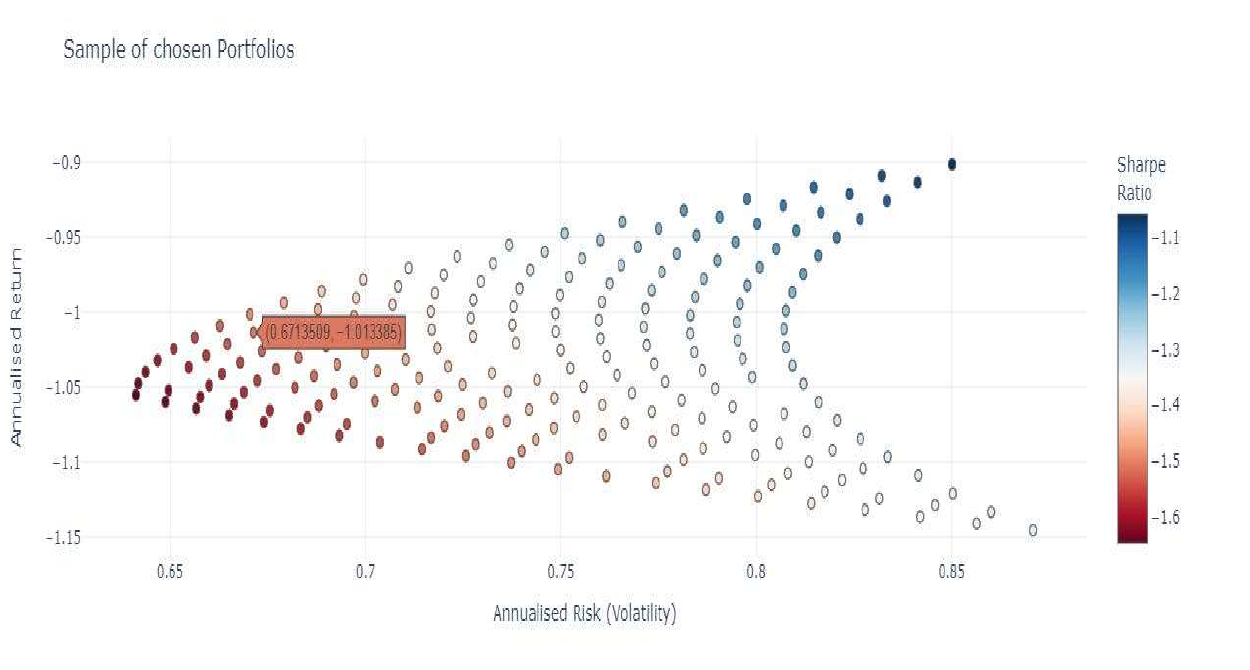
\includegraphics[width=0.98\textwidth]{../figures/portfolio_risk_return_plotly_clean.png}
\caption{Return versus risk for different cryptocurrency portfolios}
\end{figure}

\begin{figure}[H]
\centering
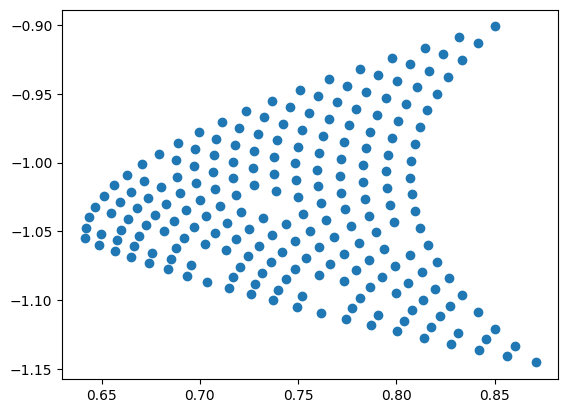
\includegraphics[width=0.88\textwidth]{../figures/notebook_cell16_output0.png}
\caption{Return versus risk for different cryptocurrency portfolios}
\end{figure}

By optimizing the Sharpe ratio, we find that the best portfolio composition consists of 100 percent Ripple and zero percent of the two other assets. Given the returns and price volatilities of the three cryptocurrencies during 2022, this result is reasonable because Ripple provides the best combination of return and volatility. Finally, a CSV file was created containing the different portfolio weights, return, variance, and Sharpe ratio for each portfolio.

\section*{Question 3}

\subsection*{Parts (a) and (b)}
Bitcoin price data for the previous year were downloaded. Moving averages from 5 days to 100 days were calculated. The goal was to determine which moving-average crossover, interpreted as a buy or sell signal, produced the highest trading profit.

To compare the profitability of different trading strategies, the problem was defined as follows: if there is a buy signal on a given day, the wealth-change ratio is equal to the ratio of the next day's Bitcoin price to today's Bitcoin price. The best strategy was obtained from the crossover of the 85-day and 80-day moving averages. Under this strategy, there were 59 buy signals and 305 sell signals.

If we follow the buy and sell signals generated by this strategy, wealth increases by approximately 4.18 percent during 2022. In the case with transaction costs, the answer is similar, except that the wealth increase is equal to 4.11 percent.

\section*{Code and Reproducibility Note}
The original Python code is preserved in the Jupyter notebook included with this project. A plain Python script extracted from the notebook is also provided in the repository. The analysis uses Yahoo Finance data, so the results may change slightly if the data source is updated or adjusted.

\end{document}
